\chapter{Fundamentação teórica}\label{cap:background}

\section{Representando poses no espaço}

\subsection{Transformações elementares}

\subsection{Transformações homogêneas}

\section{Cinemática Direta}

O problema da cinemática em manipuladores consiste em descrever o movimento do
manipulador sem considerar as forças e torques atuantes sob o mesmo
tratando-se, portanto, de uma descrição puramente geométrica. Neste contexto,
uma pergunta natural que surge é como podemos determinar a posição e orientação
do efetuador final na cadeia cinemática dado um conjunto arbitrário de ângulos
articulados. Este problema é conhecido na robótica como a cinemática direta de
um manipulador e pode ser facilmente resolvido se associarmos a cada corpo
rígido da cadeia um sistema de coordenadas (\emph{frame}), expressando também
as relações entre esses \emph{frames} como transformações homogêneas. A pose do
efetuador final fica determinada através de uma série de multiplicações
matriciais. A colocação de \emph{frames} pode ser feita de maneira sistemática
através da utilização da convenção de Denavit-Hartenberg a qual fornece uma
abordagem concisa para representar a estrutura geométrica do manipulador.

\subsection{Cadeias cinemáticas}

Na robótica, uma cadeia cinemática pode ser definida como uma série de corpos
rígidos, também denominados \emph{elos}, conectados por \emph{juntas} que
permitem um movimento relativo das diferentes partes móveis de um manipulador.
Cadeias cinemáticas formam a base do estudo de manipuladores robóticos e
geralmente são representadas através de um grafo onde seus nós constituem os
elos e as arestas as juntas.

Dependendo da topologia desse grafo, podemos classificar uma cadeia cinemática
de diferentes formas. Numa cadeia serial aberta seu grafo consiste numa árvore
onde cada nó possui apenas um único filho e o nó terminal da árvore usualmente
representa o efetuador final (onde uma pinça ou garra robótica ficaria
acoplada, por exemplo). Outros casos incluem grafos com ramificações (existe
mais de um nó terminal) onde denominamos de cadeia paralela ou quando há a
presença de ciclos onde temos uma cadeia fechada. Neste trabalho, iremos nos
limitar à análise de cadeias abertas, as mais comuns no âmbito de manipuladores
robóticos utilizados em aplicações industriais.

Os tipos de juntas presentes no cadeia também são importantes na definição do
alcance e natureza do movimento do manipulador. As mais simples são as juntas
prismáticas e de revolução, cada uma introduzindo um único grau de liberdade ao
sistema. Juntas prismáticas permitem o movimento translacional ao longo de uma
única direção enquanto que juntas de revolução possibilitam um movimento
rotacional ao redor de um eixo específico.

Ademais das juntas básicas, tipos mais complexos incluem juntas esféricas, que
introduzem dois graus de liberdade (rotação ao redor de dois eixos
perpendiculares) e punhos esféricos, compostos por três juntas revolutas
dispostas ortogonalmente, introduzindo três graus de liberdade ao sistema. Vale
ressaltar que independente da complexidade da junta, a maior parte pode ser
reduzida a uma combinação dos dois tipos mais simples tornando suficiente a
descrição de cadeias cinemáticas por meio de uma combinação de juntas
prismáticas ou de revolução.

Um manipulador robótico com $n$ juntas terá $n + 1$ elos, uma vez que cada
junta conecta exatamente dois elos. Iremos enumerar as juntas de $1$ até $n$ e
elos de $0$ a $n$ sendo que o elo de número $0$ representará a base do
manipulador e elo $n$ seu efetuador final. De acordo com essa convenção a junta
$i$ conecta os elos $i - 1$ ao $i$ e tem sua posição fixa com respeito ao elo
anterior. Quando a junta $i$ é atuada, o elo $i$ se movimenta de modo que a
base permanece fixa independente de qual junta é movimentada.

Iremos associar à $i$-ésima junta uma variável $q_i$ representando no caso de
uma junta de revolução o ângulo de rotação e no caso de uma junta prismática o
deslocamento linear:

\begin{equation}
    q_i =
    \begin{cases}
        \theta_i & \text{se a junta $i$ é de revolução} \\
        d_i      & \text{se a junta $i$ é prismática}   \\
    \end{cases}
\end{equation}

A análise cinemática é feita anexando ao elo $i$ da cadeia o sistema de
coordenadas $o_i x_i y_i z_i$. O \emph{frame} $o_0 x_0 y_0 z_0$ associado à base do
manipulador é denominado \emph{frame} da base, inercial ou do mundo. Se
$A_i(q_i)$ é a matriz de transformação homogênea que fornece a posição e
orientação de $o_i x_i y_i z_i$ com relação a $o_{i-1} x_{i-1} y_{i-1} z_{i-1}$ então
podemos dizer que a mesma é função unicamente da variável $q_i$ de modo que:

\begin{equation}
    A(q_i) = A_i = \begin{bmatrix}
        R^{i-1}_i & o^{i-1}_i \\
        0         & 1
    \end{bmatrix}
\end{equation}

Dessa forma, para $i < j$, a matriz $T_j^i$ dada por:

\begin{equation}
    T_j^i = A_{i+1} \cdots A_j = \begin{bmatrix}
        R^i_j & o^i_j \\
        0     & 1
    \end{bmatrix}
\end{equation}

expressa a orientação $R^i_j$ e posição $o^i_j$ de $o_j x_j y_j z_j$ com relação a
$o_i x_i y_i z_i$. Vale ressaltar que a matriz $R^i_j$ é calculada através da
multiplicação matricial:

\begin{equation}
    R^i_j = R^i_{i+1} \cdots R^{j-1}_j
\end{equation}

e o vetor de posição utilizando-se a seguinte equação recursiva:

\begin{equation}
    o^i_j = o^i_{j-1} + R^i_{j-1}o^{j-1}_j
\end{equation}

O problema da cinemática direta pode ser então formulado como o simples cálculo
da matriz $T^0_n$ que expressa a pose do efetuador final com relação ao
\emph{frame} da base:

\begin{equation}\label{eq:fkine}
    T^0_n = A_1 A_2 \cdots A_n = \begin{bmatrix}
        R^0_n & o^0_n \\
        0     & 1
    \end{bmatrix}
\end{equation}

Tendo em vista a infinidade de possibilidades de se anexar os \emph{frames} em
cade elo, para poder calcular as matrizes $A_i$ de forma mais precisa, vamos
estabelecer uma convenção utilizando para isso os parâmetros introduzidos por
Denavit e Hartenberg.

\subsection{Convenção de Denavit-Hartenberg}

A fixação de frames em cada elo pode ser feita de maneira arbitrária para se
obter as matrizes de transformação $A_i$, permitindo assim o cálculo da
cinemática direta. Contudo, o processo de determinação das mesmas matrizes para
um manipulador com $n$ elos começa a ser tornar cada vez mais complexo a medida
que $n$ cresce. A a convenção de Denavit-Hartenberg consiste numa abordagem
sistemática para a obtenção das matrizes $A_i$ de modo a representar a relação
entre frames consecutivos da forma mais concisa o possível além de propiciar
uma padronização de como pesquisadores descrevem a estrutura cinemática de um
manipulador robótico.

De maneira geral, para especificar a matriz de transformação homogênea seriam
necessários 6 parâmetros: três deslocamentos para a componente de translação e
três ângulos para a rotação. Na convenção de Denavit-Hartenberg, a matriz de
transformação $A_i$ associada ao $i$-ésimo elo é descrita através de apenas 4
parâmetros. Isso é obtido através da introdução de duas restrições na colocação
dos frames em cada elo:

\begin{itemize}
    \item (\textbf{DH1}) $x_i$ intersecta o eixo $z_{i-1}$
    \item (\textbf{DH2}) $x_i$ é perpendicular o eixo $z_{i-1}$
\end{itemize}

adicionar figura dh

O cálculo da matriz $A_i$ fica condicionado à determinação dos parâmetros:
$\theta_i$ (joint angle), $d_i$ (link offset), $a_i$ (link length) e $\alpha_i$
(link twist). Como $A_i$ é função da única variável da junta, três parâmetros
são sempre fixos, dependendo apenas da geometria existente entre os frames,
enquanto o quarto parâmetro é livre: $\theta_i$, no caso de uma junta de
revolução e $d_i$, no caso de uma junta prismática. Em posse dos parâmetros
obtidos para cada par de elos consecutivos, o cálculo da matriz $A_i$ é obtido
através da relação:

\begin{align}
    A_i & = Rot_z(\theta_i) \cdot Trans_z(d_i) \cdot Trans_x(a_i) \cdot Rot_x(\alpha_i)             \\
    A_i & = \begin{bmatrix}
                c_{\theta_i} & -s_{\theta_i} & 0 & 0 \\
                s_{\theta_i} & c_{\theta_i}  & 0 & 0 \\
                0            & 0             & 1 & 0 \\
                0            & 0             & 0 & 1
            \end{bmatrix} \begin{bmatrix}
                              1 & 0 & 0 & 0   \\
                              0 & 1 & 0 & 0   \\
                              0 & 0 & 1 & d_i \\
                              0 & 0 & 0 & 1
                          \end{bmatrix} \notag                                                    \\
        & \phantom{=} \times \ \ \begin{bmatrix}
                                     1 & 0 & 0 & a_i \\
                                     0 & 1 & 0 & 0   \\
                                     0 & 0 & 1 & 0   \\
                                     0 & 0 & 0 & 1
                                 \end{bmatrix} \begin{bmatrix}
                                                   1 & 0            & 0             & 0 \\
                                                   0 & c_{\alpha_i} & -s_{\alpha_i} & 0 \\
                                                   0 & s_{\alpha_i} & c_{\alpha_i}  & 0 \\
                                                   0 & 0            & 0             & 1
                                               \end{bmatrix} \notag                 \\
    A_i & = \begin{bmatrix}
                c_{\theta_i} & -s_{\theta_i}c_{\alpha_i} & s_{\theta_i}s_{\alpha_i}  & a_i c_{\theta_i} \\
                s_{\theta_i} & c_{\theta_i}c_{\alpha_i}  & -c_{\theta_i}s_{\alpha_i} & a_i s_{\theta_i} \\
                0            & s_{\alpha_i}              & c_{\alpha_i}              & d_i              \\
                0            & 0                         & 0                         & 1
            \end{bmatrix} \label{eq:dh-matrix}
\end{align}

onde $c_{\cdot}$ e $s_{\cdot}$ denotam $\cos(\cdot)$ e $\sin(\cdot)$,
respectivamente. A tabela~\ref{tab:dh-parameters} descreve de maneira detalhada
a definição de cada parâmetro de Denavit-Hartenberg.

\begin{table}[htbp]
    \centering
    \begin{tabular}{c c}
        \toprule
        \textbf{Parâmetro} & \textbf{Definição}                                                                                     \\
        \midrule
        $\theta_i$         & \makecell[l]{O ângulo entre os eixos $\mathbf{x}_i$ e $\mathbf{x}_{i+1}$ em torno do eixo $\mathbf{z}_{i-1}$}      \\
        \midrule
        $d_i$              & \makecell[l]{A distância da origem do sistema de coordenadas $\{i\}$                                   \\ até o eixo $\mathbf{x}_{i+1}$ ao longo do eixo $\mathbf{z}_i$} \\
        \midrule
        $a_i$              & \makecell[l]{A distância entre os eixos $\mathbf{z}_i$ e $\mathbf{z}_{i+1}$ ao longo do eixo $\mathbf{x}_{i+1}$;   \\ para eixos que se intersectam, é paralela a $\mathbf{z}_i \times \mathbf{z}_{i+1}$} \\
        \midrule
        $\alpha_i$         & \makecell[l]{O ângulo entre o eixo $\mathbf{z}_i$ e o eixo $\mathbf{z}_{i+1}$ em torno do eixo $\mathbf{x}_{i+1}$} \\
        \bottomrule
    \end{tabular}
    \caption{Descrição dos parâmetros Denavit-Hartenberg}\label{tab:dh-parameters}
\end{table}

\subsection{Cinemática direta de um braço planar}

Um braço planar é um tipo de manipulador serial cujo espaço de trabalho se
limita a um plano. A figura~\ref{fig:3r-planar-arm} mostra um braço planar do
tipo 3R, o qual possui três elos e três juntas de revolução acoplados em série.
A escolha da colocação do frame da base \(o_0x_0y_0z_0\) é totalmente
arbitrária e ao tomar como indicado na figura (com o eixo \(z\) apontando para
fora do papel) a fixação dos frames subsequentes na cadeia cinemática fica
restrita a convenção de Denavit-Hartenberg adotada. A tabela DH para esse
manipulador é dada por:

\begin{table}[htbp]
    \centering
    \begin{tabular}{c c c c c}
        \toprule
        \textbf{Elo} & \(\theta\) & \(d\) & \(a\) & \(\alpha\) \\
        \midrule
        1            & \(\theta_1\) & 0       & \(a_1\) & 0            \\
        2            & \(\theta_2\) & 0       & \(a_2\) & 0            \\
        3            & \(\theta_3\) & 0       & \(a_3\) & 0            \\
        \bottomrule
    \end{tabular}
    \caption{Parâmetros DH para o braço planar 3R da figura~\ref{fig:3r-planar-arm}.}\label{tab:dh-parameters-planar-arm}
\end{table}

Dados os valores fixos \(a_i\) que indicam o comprimento do elo \(i\), as
únicas variáveis livres no cálculo da cinemática direta são os ângulos das
juntas ($q_i = \theta_i$), desse modo, vamos denotar \(\theta_1 + \theta_2 =
\theta_{12}\), \(\cos(\theta_1 + \theta_2) = c_{12}\) e assim por diante. Para
\(i = 1, 2, 3\) as matrizes $A_i$ são calculadas com o auxílio da equação~\ref{eq:dh-matrix}:

\begin{figure}
    \centering
    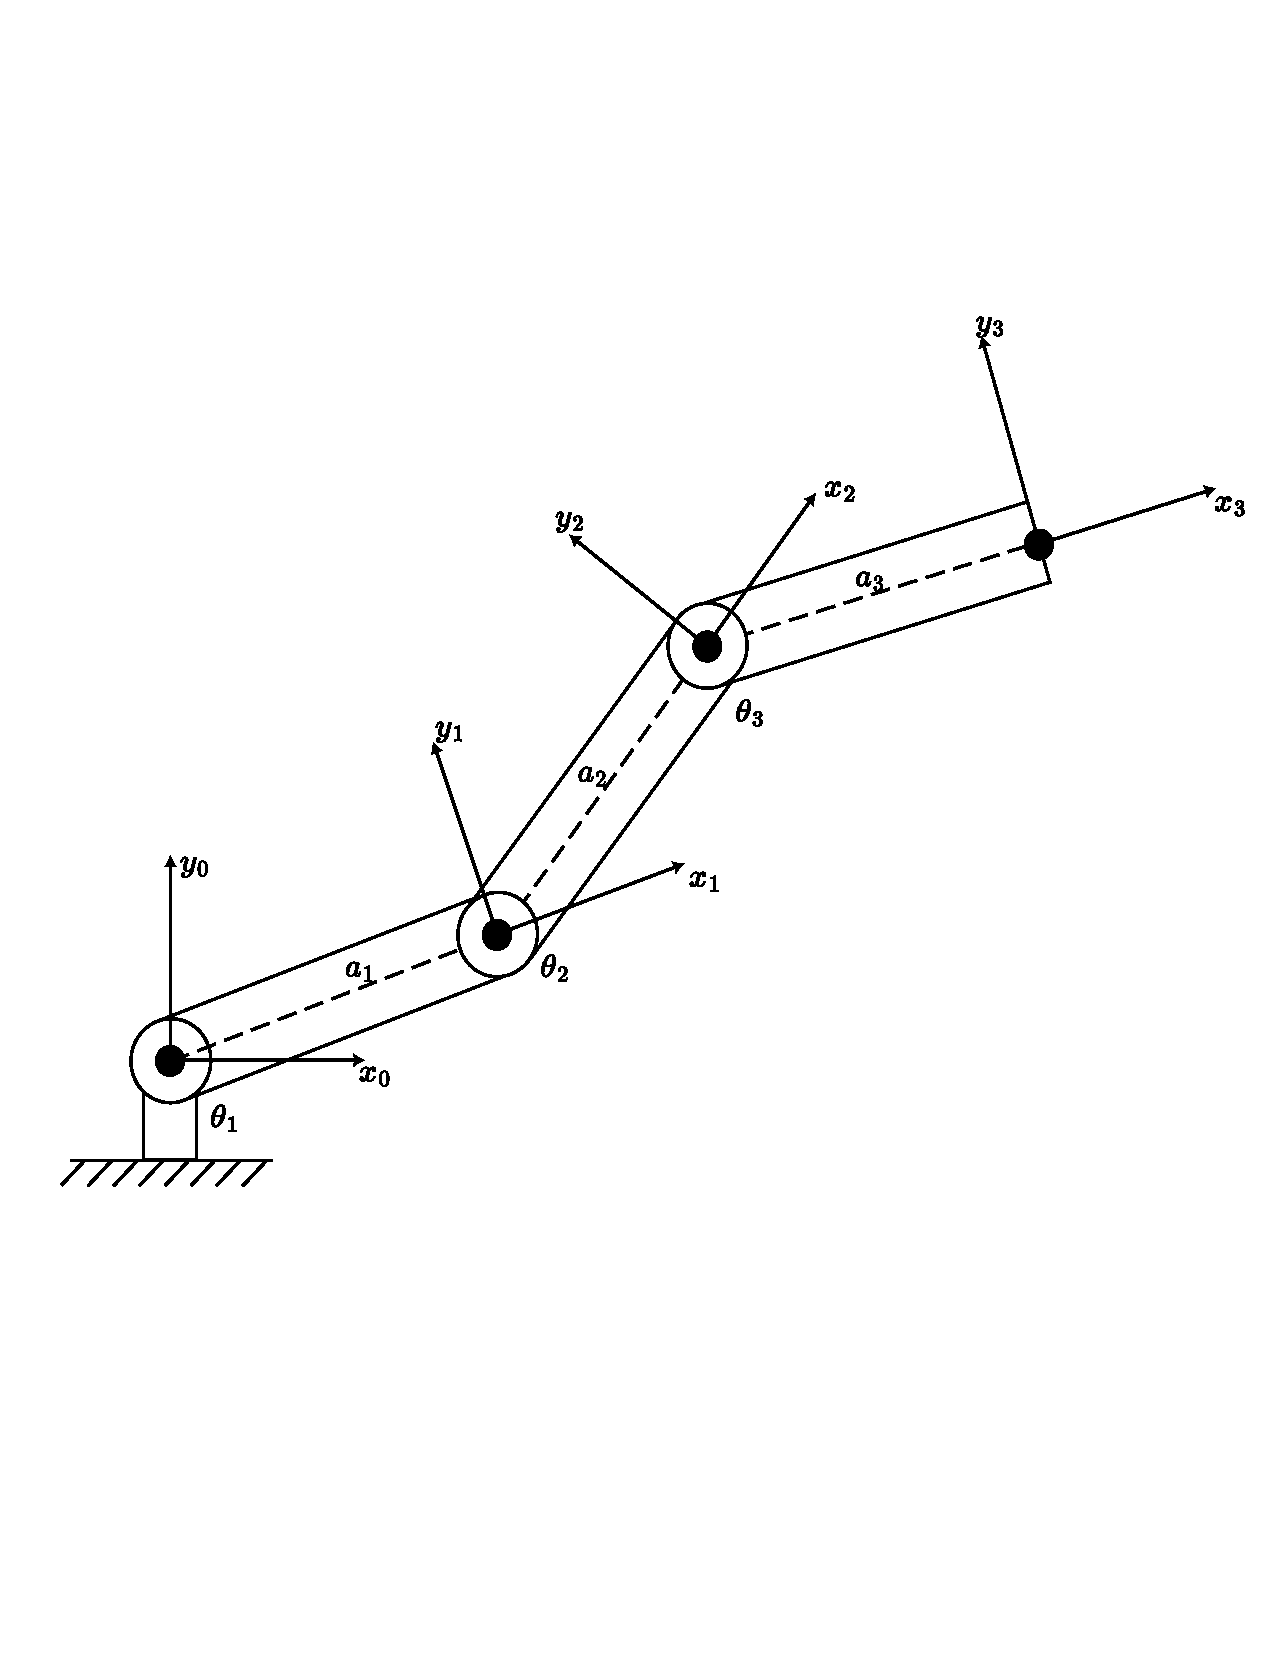
\includegraphics[width=0.8\linewidth]{export.pdf} % Adjust the width as needed
    \caption{Braço planar do tipo 3R.}\label{fig:3r-planar-arm}
\end{figure}

\begin{equation}
    \mathbf{A}_i = \begin{bmatrix}
        c_i & -s_i & 0 & a_i c_i \\
        s_i & c_i  & 0 & a_i s_i \\
        0   & 0    & 1 & 0       \\
        0   & 0    & 0 & 1
    \end{bmatrix}
\end{equation}

Já para as matrizes \(T^0_i\), utilizamos a equação~\ref{eq:fkine}:

\begin{equation}
    \mathbf{T}^0_1 = \mathbf{A}_1
\end{equation}

\begin{equation}
    \mathbf{T}^0_2 = \mathbf{A}_1 \cdot \mathbf{A}_2 = \begin{bmatrix}
        c_{12} & -s_{12} & 0 & a_1c_1 + a_2c_{12} \\
        s_{12} & c_{12}  & 0 & a_1s_1 + a_2s_{12} \\
        0      & 0       & 1 & 0                  \\
        0      & 0       & 0 & 1
    \end{bmatrix}
\end{equation}

\begin{equation}
    \mathbf{T}^0_3 = \mathbf{A}_1 \cdot \mathbf{A}_2 \cdot \mathbf{A}_3 = \begin{bmatrix}
        c_{123} & -s_{123} & 0 & a_1c_1 + a_2c_{12} + a_3c_{123} \\
        s_{123} & c_{123}  & 0 & a_1s_1 + a_2s_{12} + a_3s_{123} \\
        0       & 0        & 1 & 0                               \\
        0       & 0        & 0 & 1
    \end{bmatrix}
\end{equation}

As três primeiras entradas da última coluna da matriz \(T^0_3\) dão a posição
\(\mathbf{\xi} = {\left[ \xi_x \ \xi_y \ \xi_z \right]}^{\top}\) do efetuador final em função
da configuração do manipulador. Note que $\xi_z = 0$ quaisquer que sejam os
ângulos das juntas pois, como esperado, o manipulador é planar. Além disso,
analisando a componente de rotação, fica evidente que a orientação do efetuador
final com relação ao frame da base é dada pela soma dos ângulos das juntas:
$\psi = \theta_{123}$.

\section{Cinemática Inversa}

\subsection{Cinemática Diferencial}

\subsection{Singularidades Cinemáticas}

\subsection{Resolved Rate Control}

\section{Manipuladores redundantes}

\subsection{A Pseudo-Inversa da Jacobiana}

\subsection{Resolução de Redundância}

% Gerando movimentos no espaço nulo da jacobiana
